%; whizzy chapter -dvi
% -initex iniptex -latex platex -format platex -bibtex jbibtex -fmt fmt
% 以上 whizzytex を使用する場合の設定。

%     Tokyo Debian Meeting resources
%     Copyright (C) 2012 Junichi Uekawa
%     Copyright (C) 2011, 2015, 2020 Nobuhiro Iwamatsu

%     This program is free software; you can redistribute it and/or modify
%     it under the terms of the GNU General Public License as published by
%     the Free Software Foundation; either version 2 of the License, or
%     (at your option) any later version.

%     This program is distributed in the hope that it will be useful,
%     but WITHOUT ANY WARRANTY; without even the implied warranty of
%     MERCHANTABILITY or FITNESS FOR A PARTICULAR PURPOSE.  See the
%     GNU General Public License for more details.

%     You should have received a copy of the GNU General Public License
%     along with this program; if not, write to the Free Software
%     Foundation, Inc., 51 Franklin St, Fifth Floor, Boston, MA  02110-1301 USA

%  preview (shell-command (concat "evince " (replace-regexp-in-string "tex$" "pdf"(buffer-file-name)) "&"))

%%ここからヘッダ開始。

\documentclass[mingoth,a4paper]{jsarticle}
\usepackage{monthlyreport}
% 日付を定義する、毎月変わります。
\newcommand{\debmtgyear}{2022}
\newcommand{\debmtgmonth}{10}
\newcommand{\debmtgdate}{15}
% started from zero:
% (let ((year 2021) (month 1)) (+ (* (- year 2005) 12) month -1))
% and add 1
\newcommand{\debmtgnumber}{214}

% Needed to import pandoc-generated LaTeX documents.
% See https://stackoverflow.com/questions/40438037/tightlist-error-using-pandoc-with-markdown
\providecommand{\tightlist}{%
  \setlength{\itemsep}{0pt}\setlength{\parskip}{0pt}}

\begin{document}

\begin{titlepage}
\thispagestyle{empty}
% タイトルページ:編集必要な部分は最初のマクロに飛ばすこと

\vspace*{-2cm}
第\debmtgnumber{}回 東京エリア Debian 勉強会資料\\
\hspace*{-2cm}

\includegraphics{image-assets/dotdeb.pdf}\\
\hfill{}\debmtgyear{}年\debmtgmonth{}月\debmtgdate{}日

% ここはアップデートすること
% 全角文字にしないとフォントのサイズが合わないので注意
\rotatebox{10}{\fontsize{30}{30} {\gt KVM特集}}\\

\vspace*{-2cm}
\hfill{}
\includegraphics[height=6cm]{image-assets/openlogo-nd.eps}
\end{titlepage}

\newpage

\begin{minipage}[b]{0.2\hsize}
 \definecolor{titleback}{gray}{0.9}
 \colorbox{titleback}{\rotatebox{90}{\fontsize{80}{80} {\gt デビアン勉強会} }}
\end{minipage}
\begin{minipage}[b]{0.8\hsize}
\hrule
\vspace{2mm}
\hrule
\begin{multicols}{2}
\tableofcontents
\end{multicols}
\vspace{2mm}
\hrule
\end{minipage}

\dancersection{最近のDebian関連のミーティング報告}{杉本 典充}

\subsection{2022 年 9 月度 東京エリア・関西合同Debian勉強会}

2022 年 9 月 17 日 (土) に東京エリア Debian 勉強会と関西 Debian 勉強会の合同で
オンラインによる Debian 勉強会を開催しました。参加者は 9 名でした。

% セミナー
セミナー発表は、Yosuke OTSUKI さんの「ffmpeg + GIMP と Blender で動画編集 (CLIで呼吸している人向け)」を行いました。

% 「ffmpeg + GIMP と Blender で動画編集 (CLIで呼吸している人向け)」では、 xxx

勉強会の終了後、参加者同士で Debian や OSS に関する話の情報交換を行いました。

\dancersection{事前課題}{杉本 典充}

今回の事前課題は以下です。

\begin{enumerate}
\item 使っているデスクトップ環境を教えてください
\item 使っているインプットメソッド (IM)と、かな漢字変換ソフトを教えてください
\end{enumerate}

%この課題に対して提出いただいた内容は以下です。

\begin{multicols}{2}
{\small
\begin{prework}{ ����(yy\_y\_ja\_jp) }
���ޤ���������ǤϤʤ��Ǥ���... �긵�Υ�åץȥåפǤ� /boot �ˤ� ext2
 ����¾�ˤ� ext3���Ƕ�ȤäƤ���ǥ����ȥåפǤ� /boot �ˤ� ext3 ����¾
 �ˤ� LVM ��� ext4 ��ȤäƤ��ޤ���
\end{prework}

\begin{prework}{ �����ϥ� }
�ǥե���Ȥ�ext3����
�����ǥե���ȤΤޤޡ�
(NTFS���VM���᡼�����ext3�⤢�뤱��)
\end{prework}

\begin{prework}{ yos.takahashi }
ext3/4���˻ȤäƤޤ���ext3�Υǡ�������١����ˤĤ�������Linux2011ǯ1���˼�ɮ���ޤ�����
\end{prework}

\begin{prework}{ MATOHARA }
����inode �ϳ���������Ƥ���inode ��ưŪ�˳�����Ƥ���XFS �����򤹤뤳
 �Ȥ�¿���Ǥ���NILFS �Ͼ�����Ƥߤ��ΤǤ�����mount ���˰ʲ��Τ褦�ʥ��
 ���������ФƤޤ��ݤ��ʤȻפ��ޤ�����
\begin{commandline}
$ sudo mount /dev/sdb1 /mnt
mount.nilfs2: WARNING! - The NILFS on-disk format may change at any time.
mount.nilfs2: WARNING! - Do not place critical data on a NILFS filesystem. 
\end{commandline}
����¾NotePC �Ǥ�dm-crypt �ξ�˥ե����륷���ƥ���֤��ưŹ沽�����ꡢ
 eCryptfs �ǰŹ沽�����ꤷ�Ƥ��ޤ����񤭹��߻���CPU �򤫤ʤ���񤷤ޤ��ġ�
\end{prework}

\begin{prework}{ ��ޤ� }
��ext2-$>$reiserfs-$>$jfs-$>$xfs-$>$reiserfs-$>$ext3�ȻȤäƤ��ޤ�����

����:
\begin{itemize}
 \item reiserfs: ���ե������¿���ե�����Υ������������ӥ��Ӥ��Ƥ��ɤ���
       �����������դȤ����ⵤ�������θ�μ�žȬ�ݥ����ɤˡ�����
 \item jfs: ����v1.0��̾��ä�IBM���ꥨ�ʥ��������ˤ�xfs��ƨ��
 \item xfs: fsck==true�˴�ư����������ǯ�Ȥä���ΤΥޥ�����Ĵ����0byte
       �ե��������������Ѥ���줺ƨ����
\end{itemize}
������reiser4��Ķ���Ԥ��뤦���ˤ��줬�����ʤäơ����ext3�˸��경��htree�����ä������⤦Ŵ�Ĥʤ鲿�Ǥ⤤���Ǥ��������Ȥ����Ĥ�nilfs�ʤɤ˼��Ф��Ƥ��ޤ���ext3�������noatime���٤Ǥ����������aufs���碌�Ƽ�ʬ���Ȥ��Ȥ� *strap �Ķ��򥯥����˥󥰤��Ƥ��ޤ����¸����ƥ��Ȥ������Ǥ�����Ǥ���USB�����ư�Ǥ�ͭ�ѡ�

���LVM�ǤϤʤ�MD��Ȥäƾ�Ĺ���ܥХå����åפ򤷤Ƥ��ޤ���
 MD(sda,sdb,sdc)�ǹ��ۤ����̾��MD(����)�Dz�ư���Хå����åפλ���
 attach/detach�򤹤롣�֥��å���٥�ʤΤǥꥫ�Х��FSǤ���Ǥ��������̤�
 �������¾����ˡ���ʤ�������
\end{prework}

\begin{prework}{ henrich }
�ȤäƤ���֤�NTFS��Ĺ���󤸤�ʤ��Ǥ����͡����졣
�����Ρ����Ѥο������ǥ�������ext4�ǥե����ޥåȤ��ޤ����������㤤��Ƚ��ʤ��Ȥ����������Ƥ��ޤ���
\end{prework}

\begin{prework}{ emasaka }
�Ĥ뤷��FS��ȤäƤޤ�
\end{prework}

\begin{prework}{ �ܾ� }
ext3����Ѥ��Ƥ��ޤ����ä��Ѥ�ä����ȤϤ��Ƥ��ޤ���
FS����ʤ��Ǥ������Ƕ�Lenny��2TB��HDD��Ȥä���parted�äƤλȤ��ƶä��ޤ�����
\end{prework}

\begin{prework}{ ����@������ }
���������Ū�˳��Ѥ��Ƥ���ե����륷���ƥ��ReiserFS�Ǥ���
�Ż��ǻȤäƤ�Ķ���ext3�Ǥ�����ext3���Ÿ������ǥ��㡼�ʥ뤬
����Ʋ��Ǥ������ηи��ʸŤ������ͥ�Ǥ���...�ˤ����ꡢ
���ޤ꿮�Ѥ��Ƥ��ޤ���
�����ReiserFS�Ķ��ǤϤ���ޤǤνꤤ���ʤ��Ÿ����ڤä��ꡢ
�Ƥ�HDD�����줫�����ꤷ�Ƥ��ﳲ����ä��и���̵���Τǡ�
��³Ū�˻ȤäƤ��ޤ���
��ǯ����ReiserFS�Υᥤ��ȯ��(Hans Reiser)�����ᤵ��Ƥ��ޤ������ƥʥ󥹤��ۤ��Ƥ��ޤ�����
�����������θ��ReiserFS��¾�γ�ȯ�Ԥˤ���³�����ݼ餵��Ƥ���Τǡ��¿����ޤ�����
\end{prework}

\begin{prework}{ nozzy123nozzy }
\begin{enumerate}
 \item LVM�ˤĤ��Ƥϡ�CentOS5.5��Ƴ�������Τ��Τޤޤ����Ѥ��Ƥޤ�����
       ���������ƥब��äƤ���Volume̾�ϥǥե���Ȥ�����ȡʼºݤˤ�
       kickstart�ˤơˤ��ѹ����ƻȤäƤޤ����ʾ㳲���Υ���١����˺��뤿
       ���
\item ext3�ˤĤ��Ƥϡ�debian-sid�����Τޤ޻��ꤷ�Ƥ����Τ򤽤Τޤ޻Ȥ�
      �Ƥ����ꤷ�ޤ���relatime, noatime ���餤�Ͼ����ɲä��Ƥߤ����ʡ���
      �ϻפäƤޤ���
\end{enumerate}
\end{prework}

\begin{prework}{ �ޤ��������ؤ� }
\begin{itemize}
 \item Debian�Ǥ��ä˶Ťä����Ȥ�����ext3��ȤäƤޤ������ۥޥ����qcow2
       ���᡼���ǥ��������ѻ��ʳ��ϡ�LVM�ϻȤäƤޤ���
 \item �����ǰ����ü�ʤΤϡ��������DHCP�������Ѥ�Armadillo-J�ǻȤäƤ�
       ��JFFS�Ǥ����ǥե���ȤΥե����०�����Ǥϥ�֡��Ȥ�����������
       �ƽ��������Ƥ��ޤ��Τǡ�RAM�ΰ�˽񤭤��ߡ��Ÿ��ڤäƤ�ä��ʤ�
       ���������Ǥ���Debian��udhcp�Υ������ѥå���������ӥ�ɤ��ƻȤäƤޤ���
       \footnote{\url{http://d.hatena.ne.jp/mkouhei/20080601/1212330630}}
 \item ��Debian���ߤǡ���ʬ����ǰ��֥ۥåȤʤΤ�palm webOS�Ǥ��������Ubuntu��
       �������ޥ���������Τ餷���ΤǤ�����/etc/mtab�򸫤��35�Ԥ⤢�ꡢ
       ���ʤ����֤ʹ����Ǥ��͡�
\end{itemize}
\end{prework}
}
\end{multicols}

%\dancersection{Debian Trivia Quiz}{username}
%
%Debianの昨今の話題についてのQuizです。
%
%今回の出題範囲は\url{debian-devel-announce@lists.debian.org} や \url{debian-news@lists.debian.org}などに投稿された内容からです。
%
%\begin{multicols}{2}
%%; whizzy-master ../debianmeetingresume201211.tex
% $B0J>e$N@_Dj$r$7$F$$$k$?$a!"$3$N%U%!%$%k$G(B M-x whizzytex $B$9$k$H!"(Bwhizzytex$B$,MxMQ$G$-$^$9!#(B
%

\santaku
{DebConf13 $B$N3+:ECO$H3+:EF|$O!)(B}
{$BF|K\!"El5~ET(B 6$B7n(B20$BF|(B}
{$B%K%+%i%0%"(B $B%^%J%0%"(B 7$B7n(B8-14$BF|(B}
{$B%9%$%9!"%t%)!<%^%k%-%e(B 8$B7n(B11-18$BF|(B}
{3}
{$B%K%+%i%0%"$O(BDebConf12$B$N3+:ECO$G$9!#(B
DebConf13$B$O%9%$%9$N%-%c%s%WCO$G3+:E$G$9!#(B
6/20$B$O3'$5$sM=Dj$r6u$1$F$*$-$^$7$g$&!#(B}

\santaku
{$B@$3&$N(BWeb$B%5!<%P$G:G$b?M5$$N$"$k(BLinux $B%G%#%9%H%j%S%e!<%7%g%s(B(W3Techs$BD4$Y(B)$B$O!)(B}
{CentOS}
{Debian}
{Ubuntu}
{B}
{\url{http://w3techs.com/technologies/history_details/os-linux}$B$K7k2L$N%0%i%U$,$"$j$^$9!#(B
$B8=:_(B Linux $B$r;HMQ$7$F$$$k(B web $B%5!<%P$N(B 32.9\% $B$,(B Debian $B$rMxMQ$7$F$*$j!"$=$N3d9g$O8=:_$bA}2C$rB3$1$F$$$k$=$&$G$9!#(B}

\santaku
{Debian $B%+!<%M%k%A!<%`$N%a%s%P!<$G$"$j!"(Bkernel.org $B$N(B 3.2.y $B0BDjHG7ONs$N%a%s%F%J$G$b$"$k(B Ben Hutchings $B$5$s$,<!4|(B Debian $B0BDjHG$H0l=o$K=P2Y$5$l$k(B Linux $B%+!<%M%k$K(B (3.2 $B7ONs$N(B mainline $B$K$OL5$$(B) $BDI2C5!G=$,Ek:\$5$l$kM=Dj$G$"$k$H=R$Y$F$$$^$9!#(B
$BB?$/$NDI2CE@$NCf$K4^$^$l$J$$$b$N$O2?!)(B}
{PREEMPT\_RT}
{Hyper-V guest drivers$B$N6/2=(B}
{ARM64/AArch64$B%"!<%-%F%/%A%c%5%]!<%H(B}
{C}
{Hyper-V guest drivers$B$O(Bmainline kernel$B$G(B3.2$B$K$b4^$^$l$F$$$^$9$,!"$h$j2~A1$5$l$?(B3.4$B$+$i$N=$@5$,F3F~$5$l$^$9!#(B
PREEMPT\_RT$B$O%O!<%I%j%"%k%?%$%`$r<B8=$9$k$?$a$N(BPatch$B!"(B
linux-image-rt-amd64 , linux-image-rt-686-pae $B$N(Bmetapackage$B$G;HMQ$G$-$^$9!#(B
$B?7$7$$(BARM 64$B%S%C%H%"!<%-%F%/%A%c%5%]!<%H$O(Bmainline kernel 3.7$B$+$i(B}

\santaku
{Wookey$B$5$s$,%"%J%&%s%9$7$?(Balpha$BHG$N(BDebian port arm64 image$B$O!)(B}
{Debian/Ubuntu port image}
{Debian/KFreeBSD port image}
{Debian/GnuHurd port image}
{A}
{self-bootstrapp(non x86)$BBP1~$H$N$3$H$G$9!#(B\url{http://wiki.debian.org/Arm64Port}$B$G%9%F!<%?%9$,3NG'$G$-$^$9!#(B}

\santaku
{700,000$BHVL\$N%P%0$,Js9p$5$l$?F|$rEv$F$k(B700000thBugContest$B$N7k2L$,=P$^$7$?!#$=$NM=A[F|$HJs9pF|$O!)(B}
{2012/12/12$B$rM=A[$7$?(BDavidPrevot}
{$BM=A[F|(B:2013/02/04$B!"Js9pF|(B:2013/02/14}
{$BM=A[F|(B:2013/02/07$B!"Js9pF|(B:2013/02/14}
{$BM=A[F|(B:2013/02/14$B!"Js9pF|(B:2013/02/07}
{C}
{$B:G$b6a$$(B2013/02/14$B$rM=A[$7$?(BChristian Perrier$B$5$s$,Ev$F$^$7$?!#7k2L$O(B\url{http://wiki.debian.org/700000thBugContest}$B$G8x3+$5$l$F$$$^$9!#(B
$B$^$?!"(B800,000/1,000,000$BHVL\$N%P%0$,Js9p$5$l$kF|$rEv$F$k%3%s%F%9%H(B\url{http://wiki.debian.org/800000thBugContest}$B$b3+:E$5$l$F$$$^$9!#(B}

\santaku
{master.debian.org$B$,?7$7$$5!3#$K0\9T$5$l$^$7$?!#$3$l$O2?$N%5!<%P$G$7$g$&$+(B $B!)(B}
{@debian.org$B$N%a!<%k%5!<%P(B}
{$B%Q%C%1!<%8$N%^%9%?!<%5!<%P(B}
{$B%Q%C%1!<%8$N%9%]%s%5!<(B(mentor)$B$rC5$9%5!<%P(B}
{A}
{$B8E$$%5!<%P$O%G%#%9%/>c32Ey$,$"$C$?$N$G!"<wL?$HH=CG$5$l!"%G!<%?$,B;<:$9$kA0$K?7$7$$%5!<%P$K0\9T$5$l$^$7$?!#(Bftp-master.debian.org$B$O(BDebian$B$N(B official package $B%j%]%8%H%j$G$9!#%Q%C%1!<%8$N%9%]%s%5!<(B(mentor)$B$rC5$9$N$O(Bmentors.debian.net$B!#(B }

\santaku
{pbuilder$B$K(Bclang support$B$,DI2C$5$l$^$7$?!#C/$,=q$$$?%Q%C%A$G$7$g$&$+!)(B}
{Sylvestre Ledru}
{Junichi Uekawa}
{Hideki Yamane}
{C}
{Debian$B$N(BClang$B%5%]!<%H$OCe!9$H?J$s$G$$$^$9!#(B}

\santaku
{DPN - 2013$BG/(B3$B7n(B4$BF|9f$K<h$j>e$2$i$l$?F|K\$N%$%Y%s%H$O(B}
{Open Source Conference 2013 Tokyo/Spring}
{Open Source Conference 2013 Hamamatu}
{Open Source Conference 2013 Tokushima}
{A}
{\url{http://henrich-on-debian.blogspot.jp/2013/02/open-source-conference-2013-tokyospring.html} $B>\:Y$O8e$[$I!#(B}


%\end{multicols}


% % (query-replace-regexp "<.*?>" "")
% % (query-replace-regexp "^[    ]\+" "")
      
%-------------------------------------------------------------------------------
\dancersection{Debian で KVM を使う (CLIで呼吸している人向け)}{杉本 典充}
%-------------------------------------------------------------------------------

\subsection{はじめに}

自宅で使っている PC の入れ替えに伴い、Debian で KVM サーバを作りました。最近のDebian勉強会では KVM の話題はないため、まとめてみました。今回は KVM をコマンドラインで操作する CLI ツールに焦点を当ててみます。

なお、動作環境については OS は Debian GNU/Linux 11 bullseye amd64、CPU は Intel Core i5-6500T とします。


\subsection{KVM とは}

KVM (for Kernel-based Virtual Machine) とは、「仮想化拡張機能 (Intel VT または AMD-V) を含む x86 ハードウェア上の Linux 用の完全仮想化ソリューション」です\footnote{\url{https://www.linux-kvm.org/page/Main_Page}}。公式の Web サイトには x86 とだけ書いてありますが、Debian Wiki の KVM の説明ページ (\url{https://wiki.debian.org/KVM}) には、ARM 系 CPU も KVM が使えると記載があります。

コンピュータの仮想化技術は 表 \ref{table:type_of_virtualization} のように分類され、KVM は「完全仮想化(ハイパーバイザ型)」に該当します\footnote{引用元:東京エリアDebian勉強会 2013年4月 杉本典充「debootstrapを有効活用してみよう」8.1 仮想化技術について を元に一部加筆}。

\begin{table}[ht]
  \caption{仮想化技術の分類}
  \label{table:type_of_virtualization}
  \centering
  \begin{tabular}{|l|l|p{25em}|} \hline
    仮想化技術 & 実装例 & 仮想化環境の特徴 \\ \hline
    \begin{tabular}{l}完全仮想化\\(エミュレーション型)\end{tabular} & \begin{tabular}{l}QEMU\\VirtualBox\end{tabular} & 既存のOSを無修正のままゲスト環境として動作させる。ホストOSで動作する仮想化アプリケーションがエミューションする。 \\ \hline
    \begin{tabular}{l}完全仮想化\\(ハイパーバイザ型)\end{tabular} & \begin{tabular}{l}KVM\end{tabular} & 既存のOSを無修正のままゲスト環境として動作させる。CPU等の仮想化機能を使うことでホスト環境におけるオーバーヘッドを極力減らしている。 \\ \hline
    \begin{tabular}{l}準仮想化\end{tabular} & \begin{tabular}{l}Xen\end{tabular} & ホスト環境とやりとりするAPIを利用できるように修正が入ったOSをゲストOSとして動作させる方式(=既存のOSそのままでは動かない) \\ \hline
    \begin{tabular}{l}コンテナ型仮想化\end{tabular} & \begin{tabular}{l}OpenVZ\\LXC\\FreeBSD jail\\docker(筆者加筆)\end{tabular} & ホスト環境とゲスト環境は同一カーネルで動作しつつ、ホスト環境から分離したゲスト環境を提供する。  \\ \hline
  \end{tabular}
\end{table}

\subsection{KVM のインストール}

\subsubsection{KVM の動作条件確認}

KVM を利用するには仮想化機能に対応した CPU が必要です。Intel 製 CPU であれば Intel-VT、AMD 製 CPU であれば AMD-V、ARM64 系 CPU であれば Arm Virtualization Extensions\footnote{\url{https://developer.arm.com/documentation/ddi0406/c/System-Level-Architecture/The-System-Level-Programmers--Model/The-Virtualization-Extensions}} と呼ばれている機能を搭載しており、かつマザーボードの設定で有効にしている必要があります。

Intel 製 CPU または AMD 製 CPU であれば、

\begin{verbatim}$ grep -E 'vmx|svm' /proc/cpuinfo\end{verbatim}

というコマンドで仮想化機能が有効になっているか調べることができます (Intel 製 CPU の場合は vmx、AMD 製 CPU の場合は svm の文字列が出現します)。

\begin{commandline}
$ grep "model name" /proc/cpuinfo | head -n 1
model name      : Intel(R) Core(TM) i5-6500T CPU @ 2.50GHz
  
$ grep -E 'vmx|svm' /proc/cpuinfo | head -n 1
flags           : fpu vme de pse tsc msr pae mce cx8 apic sep mtrr pge mca cmov pat pse36 clflush dts acpi
mmx fxsr sse sse2 ss ht tm pbe syscall nx pdpe1gb rdtscp lm constant_tsc art arch_perfmon pebs bts rep_good
nopl xtopology nonstop_tsc cpuid aperfmperf pni pclmulqdq dtes64 monitor ds_cpl vmx smx est tm2 ssse3 sdbg
fma cx16 xtpr pdcm pcid sse4_1 sse4_2 x2apic movbe popcnt tsc_deadline_timer aes xsave avx f16c rdrand lahf_lm
abm 3dnowprefetch cpuid_fault epb invpcid_single pti tpr_shadow vnmi flexpriority ept vpid ept_ad fsgsbase
tsc_adjust bmi1 hle avx2 smep bmi2 erms invpcid rtm mpx rdseed adx smap clflushopt intel_pt xsaveopt xsavec
xgetbv1 xsaves dtherm ida arat pln pts hwp hwp_notify hwp_act_window hwp_epp
\end{commandline}

\subsubsection{KVM のカーネルモジュールの読み込み}

KVM を利用するには linux カーネルのカーネルモジュールを読み込む必要があります。Intel 製 CPUの場合は "kvm\_intel.ko"、AMD 製 CPUの場合は "kvm\_amd.ko" という名前になっています。

modprobe コマンドを実行してカーネルモジュールを読み込みます。以下は Intel 製 CPU のコマンド例となります。

\begin{commandline}
# modprobe kvm_intel
\end{commandline}

lsmod コマンドで "kvm\_intel" または "kvm\_amd" モジュールが表示されていれば必要なカーネルモジュールを読み込んでおり、KVM の動作条件を満たしています。

\begin{commandline}
# lsmod | grep kvm
kvm_intel             331776  0
kvm                   937984  1 kvm_intel
irqbypass              16384  1 kvm
\end{commandline}


\subsubsection{QEMU のインストール}

KVM 上で仮想マシンを実行する QEMU をインストールするには以下コマンドを実行します。今回は CLI 操作を目的とするため、GUI 関連のパッケージをインストールしないよう "--no-install-recommends" オプションを指定しています\footnote{\url{https://wiki.debian.org/KVM\#Installation}}。

\begin{commandline}
# apt install --no-install-recommends qemu-system libvirt-clients libvirt-daemon-system
\end{commandline}

KVM 上に仮想マシンをコマンドラインでインストールする virt-install コマンドを含む virtinst パッケージをインストールします。
libosinfo-bin パッケージには virt-install コマンドの "--os-variant" オプションに指定できる値を調べることができる osinfo-query コマンドが入っています\footnote{\$ osinfo-query os を実行すると一覧を表示します。}。

\begin{commandline}
# apt install virtinst libosinfo-bin
\end{commandline}

上記コマンドをインストールすると libvirt グループが作成されます。以降の手順で仮想マシンを操作するコマンドを紹介しますが、そのとき  libvirt グループ に所属しているユーザが仮想マシンを操作できます。自分のユーザを libvirt グループに追加しておきます。

\begin{commandline}
# adduser <youruser> libvirt
\end{commandline}


\subsubsection{KVM 上で動作する仮想マシンのネットワークの構成}

KVM 上の仮想マシンが接続するネットワーク構成は、NAT と Bridge の 2 種類があります。

\subsubsubsection{NAT 構成}

NAT 構成は、ホストマシンの中に仮想マシン同士が通信する専用の NAT ネットワークを作る構成をいい、KVM 上の仮想マシン用ネットワークのデフォルト設定になっています。NAT 構成の場合、仮想マシン用ネットワークが KVM のホストマシンの中で完結するため、開発用 PC やネットワークが頻繁に切り替わるノート PC では NAT 構成の利用が向いています。

\begin{figure}[h]
  \centering
  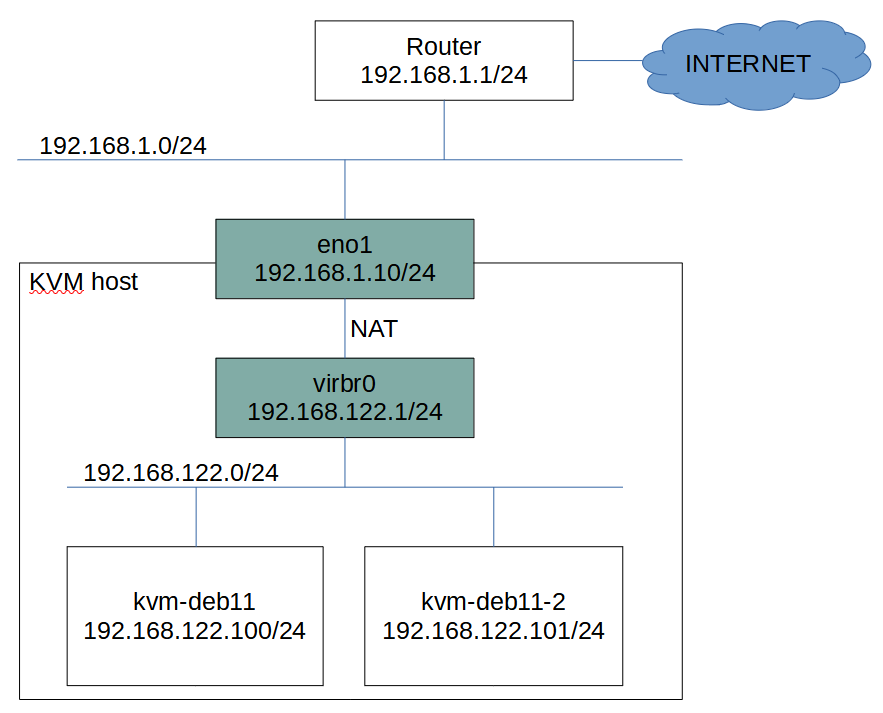
\includegraphics[scale=0.3]{image202210/kvm-network_nat.png}
  \caption{KVM ホストマシンと仮想マシンのネットワーク構成 (NAT 構成)}
  \label{fig:kvm-network_nat}
\end{figure}

以下コマンドを実行すると、仮想マシン向けのネットワークとして virbr0 インタフェースが起動します。デフォルトでは、192.168.122.0/24 のネットワークが作成され、仮想マシンから見たデフォルトゲートウェイは 192.168.122.1/24 となります。

\begin{commandline}
$ virsh --connect=qemu:///system net-start default
ネットワーク default が起動されました

$ ip addr show dev virbr0
4: virbr0: <NO-CARRIER,BROADCAST,MULTICAST,UP> mtu 1500 qdisc noqueue state DOWN group default qlen 1000
    link/ether 52:54:00:db:b9:5b brd ff:ff:ff:ff:ff:ff
    inet 192.168.122.1/24 brd 192.168.122.255 scope global virbr0
       valid_lft forever preferred_lft forever
\end{commandline}

この状態のままでは、PC の起動時に virbr0 インタフェースは自動起動しません。もし、PC の起動時に自動で virbr0 インタフェースを起動するようにしたい場合は以下コマンドを実行してください。

\begin{commandline}
$ virsh --connect=qemu:///system net-autostart default
\end{commandline}


\subsubsubsection{Bridge 構成}

Bridge 構成は、ホストマシンが接続するネットワークセグメントに仮想マシンも接続する構成のことをいいます。Bridge 構成の場合は仮想マシンの IP アドレスにホストマシンと同じセグメントの IP アドレスを割り当てるため、KVM のホストマシンとは別のホストからでも仮想マシンへ直接通信できるメリットがあります。

\begin{figure}[h]
  \centering
  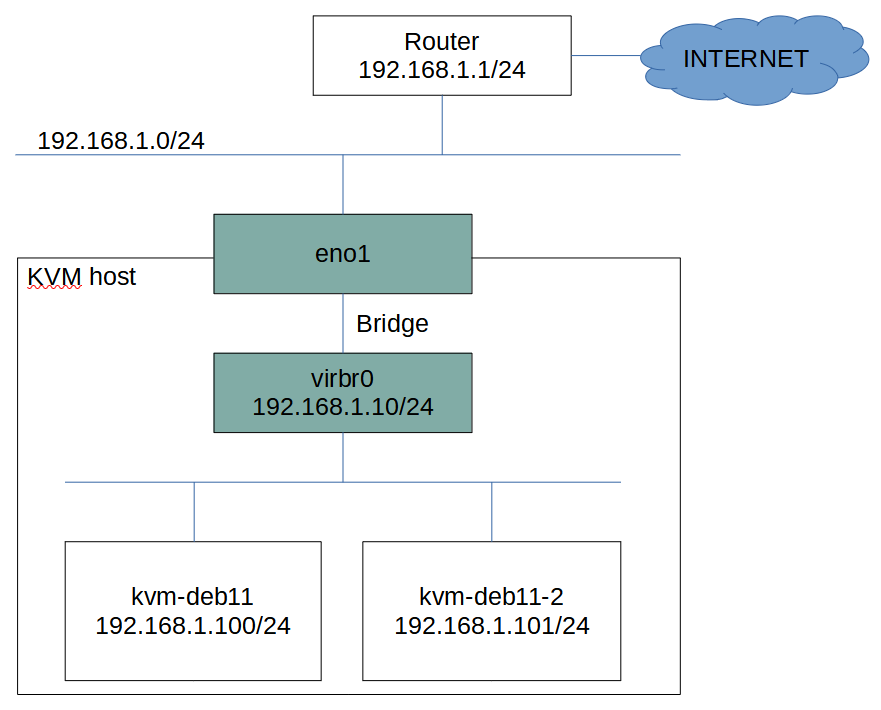
\includegraphics[scale=0.3]{image202210/kvm-network_bridge.png}
  \caption{KVM ホストマシンと仮想マシンのネットワーク構成 (Bridge 構成)}
  \label{fig:kvm-network_bridge}
\end{figure}

Bridge 構成にするには以下コマンドで追加のパッケージをインストールします。

\begin{commandline}
# apt install bridge-utils
\end{commandline}

次に有線 LAN の設定を Bridge 構成に変更します\footnote{ネットワークの設定変更をするため、ssh経由で操作している場合に設定ミスがあるとネットワークを再起動した後につながらなくなる危険性があります。できるだけホストマシンのコンソールへログインできる状況で作業する方がよいです。}。

変更前の有線 LAN で固定の IP アドレスに設定している設定ファイルは以下です。

\begin{commandline}
$ cat /etc/network/interfaces
# This file describes the network interfaces available on your system
# and how to activate them. For more information, see interfaces(5).

source /etc/network/interfaces.d/*

# The loopback network interface
auto lo
iface lo inet loopback

# The primary network interface
allow-hotplug eno1
iface eno1 inet static
  address 192.168.1.10
  netmask 255.255.255.0
  gateway 192.168.1.1
  dns-nameservers 192.168.1.1
  bridge_ports eno1
  bridge_stp off

# This is an autoconfigured IPv6 interface
iface eno1 inet6 auto
\end{commandline}

以下のようにネットワークの設定を変更して Bridge のインタフェースに IP アドレスを設定し、有線 LAN のインタフェースへ Bridge するよう紐つけます。

\begin{commandline}
$ sudo vi /etc/network/interfaces
# This file describes the network interfaces available on your system
# and how to activate them. For more information, see interfaces(5).

source /etc/network/interfaces.d/*

# The loopback network interface
auto lo
iface lo inet loopback

# The primary network interface
allow-hotplug eno1
iface eno1 inet manual

auto br0
iface br0 inet static
  address 192.168.1.10
  netmask 255.255.255.0
  gateway 192.168.1.1
  dns-nameservers 192.168.1.1
  bridge_ports eno1
  bridge_stp off

# This is an autoconfigured IPv6 interface
iface eno1 inet6 auto
\end{commandline}

設定変更を反映するため、ネットワークを再起動します。

\begin{commandline}
$ sudo systemctl restart networking
\end{commandline}

ホストマシンから wget や apt を実行して、ネットワークに接続できることを確認してみてください。


\subsection{KVM 上の仮想マシンを操作するコマンド}

\subsubsection{qemu-img コマンド}

qemu-img コマンドは、KVM 上で動作する仮想マシンの仮想ディスクを作成、変更するコマンドです。

仮想ディスクを作成するには "create" サブコマンドで作成できます。以下の例は、KVM で利用できる qcow2 形式 の 10 GB の仮想ディスクを作成します。
qcow2 形式の仮想ディスクは実際にデータを書き込んだ分だけファイルサイズが増えていくため (スパースファイル、またはスパースディスクといいます)、作成直後のファイルサイズはとても小さいです。

\begin{commandline}
# qemu-img create -f qcow2 /var/lib/libvirt/images/kvm-deb11.img 10g
Formatting '/var/lib/libvirt/images/kvm-deb11.img', fmt=qcow2 cluster_size=65536 extended_l2=off
compression_type=zlib size=10737418240 lazy_refcounts=off refcount_bits=16

# ls -lh /var/lib/libvirt/images/kvm-deb11.img
-rw-r--r-- 1 root root 193K 10月 12 23:11 /var/lib/libvirt/images/kvm-deb11.img

# file /var/lib/libvirt/images/kvm-deb11.img
kvm-deb11.img: QEMU QCOW2 Image (v3), 10737418240 bytes
\end{commandline}

qemu-img コマンドのオプションには他の仮想化ソフトが採用している仮想ディスクの形式と相互変換する "convert" サブコマンドもあります。
以下の例は、VirtualBox 向けの VDI 形式から KVM 向けの qcow2 形式へ変換するコマンドです。

\begin{commandline}
$ qemu-img convert -f vdi disk-virtualbox.vdi -O qcow2 disk-kvm.img
\end{commandline}


\subsubsection{virt-install コマンド}

\subsubsubsection{仮想マシンのOSインストールをシリアル接続したコンソールで操作して行う場合}

virt-install コマンドを使うと、KVM 上に仮想マシンをインストールすることができます。
コマンドライン環境で仮想マシンをインストールする場合は、起動した仮想マシンのコンソールへシリアル接続するようパラメータを指定します (--graphics none、--console オプション、--extra-args オプション)。以下のように virt-install コマンドを実行すると、起動した仮想マシンのコンソールで Debian インストーラの処理が始まり、キーボード入力で仮想マシンへ Debian のインストールを行うことができます。

\begin{commandline}
$ sudo virt-install \
--name kvm-deb11 \
--disk path=/var/lib/libvirt/images/kvm-deb11.img,format=qcow2,bus=virtio \
--vcpus 1 \
--ram 1024 \
--os-type linux \
--os-variant generic \
--network bridge=br0,model=virtio \
--location 'http://deb.debian.org/debian/dists/bullseye/main/installer-amd64/' \
--graphics none \
--console pty,target_type=serial \
--extra-args 'console=ttyS0,115200n8 serial'
\end{commandline}


\subsubsubsection{仮想マシンのOSインストールをpreseed機能を使って自動インストールする場合}

Debian インストーラには設定ファイルにしたがって OS を自動インストールする preseed\footnote{付録B preseed を利用したインストールの自動化 \url{https://www.debian.org/releases/bullseye/amd64/apb.ja.html}} という機能があります。virt-install コマンドのパラメータに preseed の設定ファイルを指定することで仮想マシンへ Debian を自動インストールでき、検証環境の作成や大量に仮想マシンをインストールする場合に便利です。

Debian 11 bullseye 向けの preseed 設定ファイルのサンプルは以下 URL にあります。

\begin{itemize}
\item \url{https://www.debian.org/releases/bullseye/example-preseed.txt}
\end{itemize}

preseed の設定ファイルを作成し\footnote{詳しくは、第 144 回東京エリア Debian 勉強会「preseedでDebianを自動インストール」を参照。}、/var/lib/libvirt/images/preseed.cfg としてホストマシンに置きます。そして virt-install コマンドのパラメータに "--initrd-inject" を指定すると 仮想マシンの / 直下に "--initrd-inject" で指定したファイルがコピーされます。すると、仮想マシン上で起動した Debian インストーラの処理が /preseed.cfg を検出し、シリアル接続した仮想マシンのコンソール上で Debian のインストールが自動で進んでいきます\footnote{使ったpreseedの設定ファイルは \url{https://github.com/dictoss/utils/blob/master/debian-preseed/preseed-debian11.cfg}}。

\begin{commandline}
$ sudo qemu-img create -f qcow2 /var/lib/libvirt/images/kvm-deb11-2.img 10g
  
$ sudo virt-install \
--name kvm-deb11-2 \
--disk path=/var/lib/libvirt/images/kvm-deb11-2.img,format=qcow2,bus=virtio \
--vcpus 1 \
--ram 1024 \
--os-type linux \
--os-variant generic \
--network bridge=br0,model=virtio \
--location 'http://deb.debian.org/debian/dists/bullseye/main/installer-amd64/' \
--initrd-inject=/var/lib/libvirt/images/preseed.cfg \
--graphics none \
--console pty,target_type=serial \
--extra-args 'console=ttyS0,115200n8 serial'
\end{commandline}


\subsubsection{virsh コマンド}

\subsubsubsection{virsh とは}

virsh コマンドは Debian では libvirt-clients パッケージで提供されており、仮想マシンを制御する様々なハイパーバイザーに対応するコマンドラインのフロントエンドツールです。Linux では KVM や Xen のハイパーバイザーの操作に virsh を利用することができます。

virshは、"virsh \{サブコマンド\}" のような形のコマンドを実行することで仮想マシンを制御できます。


\subsubsubsection{virsh help}

"virsh help" コマンドを実行すると、サブコマンドの一覧が表示されます。

\begin{commandline}
$ virsh help
グループ別コマンド:

 Domain Management (ヘルプのキーワード 'domain'):
    attach-device                  XML ファイルによるデバイスの接続
    attach-disk                    ディスクデバイスの接続
    attach-interface               ネットワークインターフェースの接続
    autostart                      ドメインの自動起動
    blkdeviotune                   ブロックデバイスの I/O チューニングパラメーターの設定・取得
    blkiotune                      ブロック I/O パラメーターの取得・設定
    blockcommit                    ブロックのコミット操作の開始
  (以下、省略)
\end{commandline}

また、"virsh help \{サブコマンド\}" を実行すると、サブコマンドの使い方とオプションを調べることができます。

\begin{commandline}
$ virsh help start
  名前
    start - 停止状態の(定義済み)ドメインの起動

  形式
    start <domain> [--console] [--paused] [--autodestroy] [--bypass-cache] [--force-boot] [--pass-fds <string>]
  (以下、省略)
\end{commandline}


\subsubsubsection{virsh --connect}

KVM のハイパーバイザーに接続するには "virsh --connect" を実行します。接続先を示す "qemu:///system" は URI 形式になっており、接続に利用するプロトコルを切り替えたり、リモート先のホストを指定することができます。

以下の例は、KVM のハイパーバイザーが動作しているホストマシン上からローカル接続する場合のコマンドです。

\begin{commandline}
$ virsh --connect qemu:///system
virsh にようこそ、仮想化対話式ターミナルです。

入力: 'help' コマンドのヘルプ
      'quit' 終了

virsh #
\end{commandline}

"virsh --connect" で KVM のハイパーバイザーへ接続すると以降は対話的な操作に移ります。接続中はサブコマンドのみで操作が可能になります。


\subsubsubsection{list サブコマンド}

list サブコマンドは、仮想マシンの一覧を出力することができます。オプションの指定値で一覧に表示する仮想マシンが変わります。 

単に "list" と実行した場合は起動中の仮想マシンのみ表示し、"list --inactive" と実行した場合は停止中の仮想マシンのみを表示し、"list --all" と実行した場合はすべての仮想マシンを表示します。

\begin{commandline}
virsh # list
 Id   名前        状態
--------------------------
 1    kvm-deb11   実行中
\end{commandline}

\begin{commandline}
virsh # list --inactive
 Id   名前              状態
--------------------------------------
 -    kvm-deb11-2       シャットオフ

\end{commandline}

\begin{commandline}
virsh # list --all
 Id   名前              状態
--------------------------------------
 1    kvm-deb11         実行中
 -    kvm-deb11-2       シャットオフ
\end{commandline}


\subsubsubsection{virsh edit}

edit サブコマンドは、仮想マシンの設定ファイル(XML 形式)を開き、編集することができます。edit サブコマンドを実行すると環境変数 EDITOR で指定しているエディタで XML ファイルを開きます\footnote{XML ファイルの定義は \url{https://libvirt.org/formatdomain.html} を参照。}。

\begin{commandline}
virsh # edit kvm-deb11


<domain type='kvm'>
  <name>kvm-deb11</name>
  <uuid>6dec70d3-09e5-40c6-b269-eaf20a2651d9</uuid>
  <memory unit='KiB'>1048576</memory>
  <currentMemory unit='KiB'>1048576</currentMemory>
  <vcpu placement='static'>1</vcpu>
  <os>
    <type arch='x86_64' machine='pc-i440fx-5.2'>hvm</type>
    <boot dev='hd'/>
  </os>
  (以降、省略)
\end{commandline}


\subsubsubsection{start サブコマンド}

start サブコマンドは、仮想マシンを起動することができます。start サブコマンドを実行すると仮想マシンはバックグラウンドで起動します。

\begin{commandline}
virsh # start kvm-deb11
Domain 'kvm-deb11' started
\end{commandline}

"start --console" オプションを指定すると仮想マシンの起動と同時に仮想マシンのコンソールにシリアル接続します。

\begin{commandline}
virsh # start --console kvm-deb11
Domain 'kvm-deb11' started
Connected to domain 'kvm-deb11-2'
Escape character is ^] (Ctrl + ])

 (以降、コンソールにOSの起動ログが表示される)

kvm-deb11 login:  
\end{commandline}


\subsubsubsection{virsh console}

console サブコマンドは、起動中の仮想マシンのコンソールへシリアル接続することができます。

\begin{commandline}
virsh # console kvm-deb11
Connected to domain 'kvm-deb11'
Escape character is ^] (Ctrl + ])

kvm-deb11 login:
\end{commandline}


\subsubsubsection{virsh destroy}

destroy サブコマンドは、仮想マシンを強制的に停止することができます。なお、stop サブコマンドはありません。

\begin{commandline}
virsh # destroy kvm-deb11
Domain 'kvm-deb11' destroyed
\end{commandline}


\subsubsubsection{virsh undefine}

undefine サブコマンドは、仮想マシンの登録を削除します。undefine サブコマンドにオプションを指定せずに実行した場合は仮想マシンに接続していた仮想ディスクは削除されずに残ります\footnote{仮想ディスクも一緒に削除したい場合は、--storage \{string\}、--remove-all-storage などのオプションが利用できます。}。

\begin{commandline}
virsh # undefine kvm-deb11
Domain 'kvm-deb11' has been undefined
\end{commandline}


\subsubsubsection{virsh define}

define サブコマンドは、仮想マシンの構成を定義した XML ファイルから仮想マシンを登録できます。

\begin{commandline}
virsh # define /etc/libvirt/qemu/kvm-deb11-3.xml
\end{commandline}


\subsection{おわりに}

Debian 上で KVM を使えるように設定し、virt-install コマンドや virsh コマンドを説明しました。GUI から操作するより CLI から操作した方が便利な場合もありますので、有効に活用してみてください。

\subsection{参考文献}

\begin{itemize}
\item Home - linux-kvm.org \url{http://www.linux-kvm.org/page/Main_Page}
\end{itemize}

\begin{itemize}
\item KVM - Debian Wiki \url{https://wiki.debian.org/KVM}
\end{itemize}

\begin{itemize}
\item 第 144 回東京エリアDebian勉強会「preseed で Debian を自動インストールをしてみよう」 \url{https://tokyodebian-team.pages.debian.net/pdf2016/debianmeetingresume201610-presentation-sugimoto.pdf}
\end{itemize}


% 冊子にするために、4の倍数にする必要がある。
% そのための調整
\dancersection{メモ}{}
\mbox{}\newpage
\mbox{}\newpage

\vspace*{15cm}
\hrule
\vspace{2mm}

\includegraphics[width=2cm]{image-assets/openlogo-nd.eps}
\noindent \Large \bf Debian 勉強会資料\\
\noindent \normalfont \debmtgyear{}年\debmtgmonth{}月\debmtgdate{}日 \hspace{5mm}  初版第1刷発行\\
\noindent \normalfont 東京エリア Debian 勉強会 (編集・印刷・発行)\\
\hrule
\end{document}
